\newcommand{\malwareResultsAucTable}{
    \begin{table}[H]
        \centering
        \begin{tabular}{|p{2,8cm}||P{2,4cm} P{2,4cm} P{2,4cm}|}
            \hline
            Malware Label & ALOHA\newline (M/B only) & ALOHA & Proposed\newline Model \\
            \hline
            AUC-ROC & 0.841$\pm$0.015 & 0.776$\pm$0.000 & \textBF{0.852$\pm$0.033} \\
            \hline
        \end{tabular}
        \caption[Malware Label prediction task AUC-ROC results]{AUC-ROC (Area Under Curve) of the different models for the \textbf{Malware Label} prediction task. Results were aggregated over \textBF{2} training runs with different weight initializations and minibatch orderings. Best results are shown in \textbf{bold}.} \label{tab:malware_auc}
    \end{table}
}

\newcommand{\malwareResultsAtFprTable}{
    \begin{center}
        \begin{longtable}[c]{|P{3,2cm}||P{1,8cm} P{1,8cm} P{1,8cm} P{1,8cm} P{1,8cm}|}
            \hline
            Malware Label & \multicolumn{5}{c|}{{FPR}} \\
            & $10^{-5}$ & $10^{-4}$ & $10^{-3}$ & $10^{-2}$ & $10^{-1}$ \\
            \hline
            \endfirsthead

            \caption*{\raggedright ...continued from previous page} \\
            \hline
            Malware Label & \multicolumn{5}{c|}{\textbf{FPR}} \\
            & $10^{-5}$ & $10^{-4}$ & $10^{-3}$ & $10^{-2}$ & $10^{-1}$ \\
            \hline
            \endhead

            \caption*{\raggedleft ...continued on next page} \\
            \endfoot

            \caption[Malware Label prediction task results]{Mean and standard deviation results (TPR, Accuracy, Recall, Precision and F1-Score) of the different models for the \textbf{Malware Label} prediction task at different \textbf{FPR}s (\textit{False Positive Rates}). Results were aggregated over \textBF{2} training runs with different weight initializations and minibatch orderings. Best results are shown in \textbf{bold}. Under \textbf{TPR} results are also presented the percentage reduction in mean detection error and in ROC curve standard deviation introduced by the \textit{Proposed Model} with respect to both \textit{ALOHA} model and \textit{Joint Embedding}.} \label{tab:malware_results_at_fpr} \\
            \endlastfoot

            \multicolumn{6}{|c|}{\textbf{TPR}} \\
            \hline
            ALOHA (M/B only) & \textBF{0.122$\pm$0.007} & \textBF{0.122$\pm$0.007} & \textBF{0.168$\pm$0.039} & 0.256$\pm$0.011 & 0.516$\pm$0.009 \\
            ALOHA & 0.006$\pm$0.006 & 0.006$\pm$0.006 & 0.013$\pm$0.001 & 0.064$\pm$0.026 & 0.295$\pm$0.024 \\
            Proposed Model & 0.072$\pm$0.046 & 0.072$\pm$0.046 & 0.077$\pm$0.041 & \textBF{0.271$\pm$0.075} & \textBF{0.521$\pm$0.079} \\
            \hline
            Error Reduction wrt\newline ALOHA (M/B only) & -5.7\% & -5.7\% & -10.9\% & 2.0\% & 1.0\% \\
            Error Reduction wrt\newline ALOHA & 6.6\% & 6.6\% & 6.5\% & 22.1\% & 32.1\% \\
            \hline
            Std Reduction wrt\newline ALOHA (M/B only) & -557.1\% & -557.1\% & -5.1\% & -581.8\% & -777.8\% \\
            Std Reduction wrt\newline ALOHA & -666.7\% & -666.7\% & -4000.0\% & -188.5\% & -229.2\% \\
            \hline
            \multicolumn{6}{|c|}{\textbf{Accuracy}} \\
            \hline
            ALOHA (M/B only) & \textBF{0.747$\pm$0.002} & \textBF{0.747$\pm$0.002} & \textBF{0.760$\pm$0.011} & 0.779$\pm$0.003 & 0.790$\pm$0.003 \\
            ALOHA & 0.714$\pm$0.002 & 0.714$\pm$0.002 & 0.716$\pm$0.000 & 0.724$\pm$0.007 & 0.726$\pm$0.007 \\
            Proposed Model & 0.733$\pm$0.013 & 0.733$\pm$0.013 & 0.734$\pm$0.012 & \textBF{0.783$\pm$0.021} & \textBF{0.791$\pm$0.022} \\
            \hline
            \multicolumn{6}{|c|}{\textbf{Recall}} \\
            \hline
            ALOHA (M/B only) & \textBF{0.122$\pm$0.007} & \textBF{0.122$\pm$0.007} & \textBF{0.168$\pm$0.039} & 0.256$\pm$0.011 & 0.516$\pm$0.009 \\
            ALOHA & 0.006$\pm$0.006 & 0.006$\pm$0.006 & 0.013$\pm$0.001 & 0.064$\pm$0.026 & 0.295$\pm$0.024 \\
            Proposed Model & 0.072$\pm$0.046 & 0.072$\pm$0.046 & 0.077$\pm$0.041 & \textBF{0.271$\pm$0.075} & \textBF{0.521$\pm$0.079} \\
            \hline
            \multicolumn{6}{|c|}{\textbf{Precision}} \\
            \hline
            ALOHA (M/B only) & \textBF{1.000$\pm$0.000} & \textBF{1.000$\pm$0.000} & \textBF{0.986$\pm$0.007} & \textBF{0.914$\pm$0.003} & \textBF{0.678$\pm$0.005} \\
            ALOHA & \textBF{1.000$\pm$0.000} & \textBF{1.000$\pm$0.000} & 0.899$\pm$0.010 & 0.701$\pm$0.087 & 0.543$\pm$0.021 \\
            Proposed Model & \textBF{1.000$\pm$0.000} & \textBF{1.000$\pm$0.000} & 0.981$\pm$0.019 & 0.912$\pm$0.022 & 0.675$\pm$0.033 \\
            \hline
            \multicolumn{6}{|c|}{\textbf{F1 Score}} \\
            \hline
            ALOHA (M/B only) & \textBF{0.218$\pm$0.011} & \textBF{0.218$\pm$0.011} & \textBF{0.286$\pm$0.057} & 0.400$\pm$0.013 & \textBF{0.586$\pm$0.007} \\
            ALOHA & 0.011$\pm$0.011 & 0.011$\pm$0.011 & 0.025$\pm$0.003 & 0.116$\pm$0.044 & 0.382$\pm$0.025 \\
            Proposed Model & 0.130$\pm$0.081 & 0.130$\pm$0.081 & 0.140$\pm$0.071 & \textBF{0.413$\pm$0.091} & 0.586$\pm$0.063 \\
            \hline
        \end{longtable}
    \end{center}
}

\newcommand{\malwareResultsSummaryTable}{
    \begin{table}[H]
        \centering
        \begin{tabular}{|P{3,2cm}||P{1,8cm} P{1,8cm} P{1,8cm} P{1,8cm} P{1,8cm}|}
            \hline
            \multicolumn{6}{|c|}{Malware Label (at FPR $=1\%$)} \\
            \hline
            Model & TPR & Accuracy & Precision & Recall & F1 score \\
            \hline
            ALOHA (M/B only) & 0.256$\pm$0.011 & 0.779$\pm$0.003 & \textBF{0.914$\pm$0.003} & 0.256$\pm$0.011 & 0.400$\pm$0.013 \\
            ALOHA & 0.064$\pm$0.026 & 0.724$\pm$0.007 & 0.701$\pm$0.087 & 0.064$\pm$0.026 & 0.116$\pm$0.044 \\
            Proposed Model & \textBF{0.271$\pm$0.075} & \textBF{0.783$\pm$0.021} & 0.912$\pm$0.022 & \textBF{0.271$\pm$0.075} & \textBF{0.413$\pm$0.091} \\
            \hline
        \end{tabular}
        \caption[Summary of Malware Label prediction task results]{Summary of the mean and standard deviation results of the different models for the \textbf{Malware Label} prediction task at \textbf{FPR} $=1\%$. Results were aggregated over \textBF{2} training runs with different weight initializations and minibatch orderings. Best results are shown in \textbf{bold}.} \label{tab:malware_result_summary}
    \end{table}
}

\newcommand{\malwareRocAlohaMB}{
    \begin{figure}[H]
        \vspace*{-0.5cm}
        \centering
        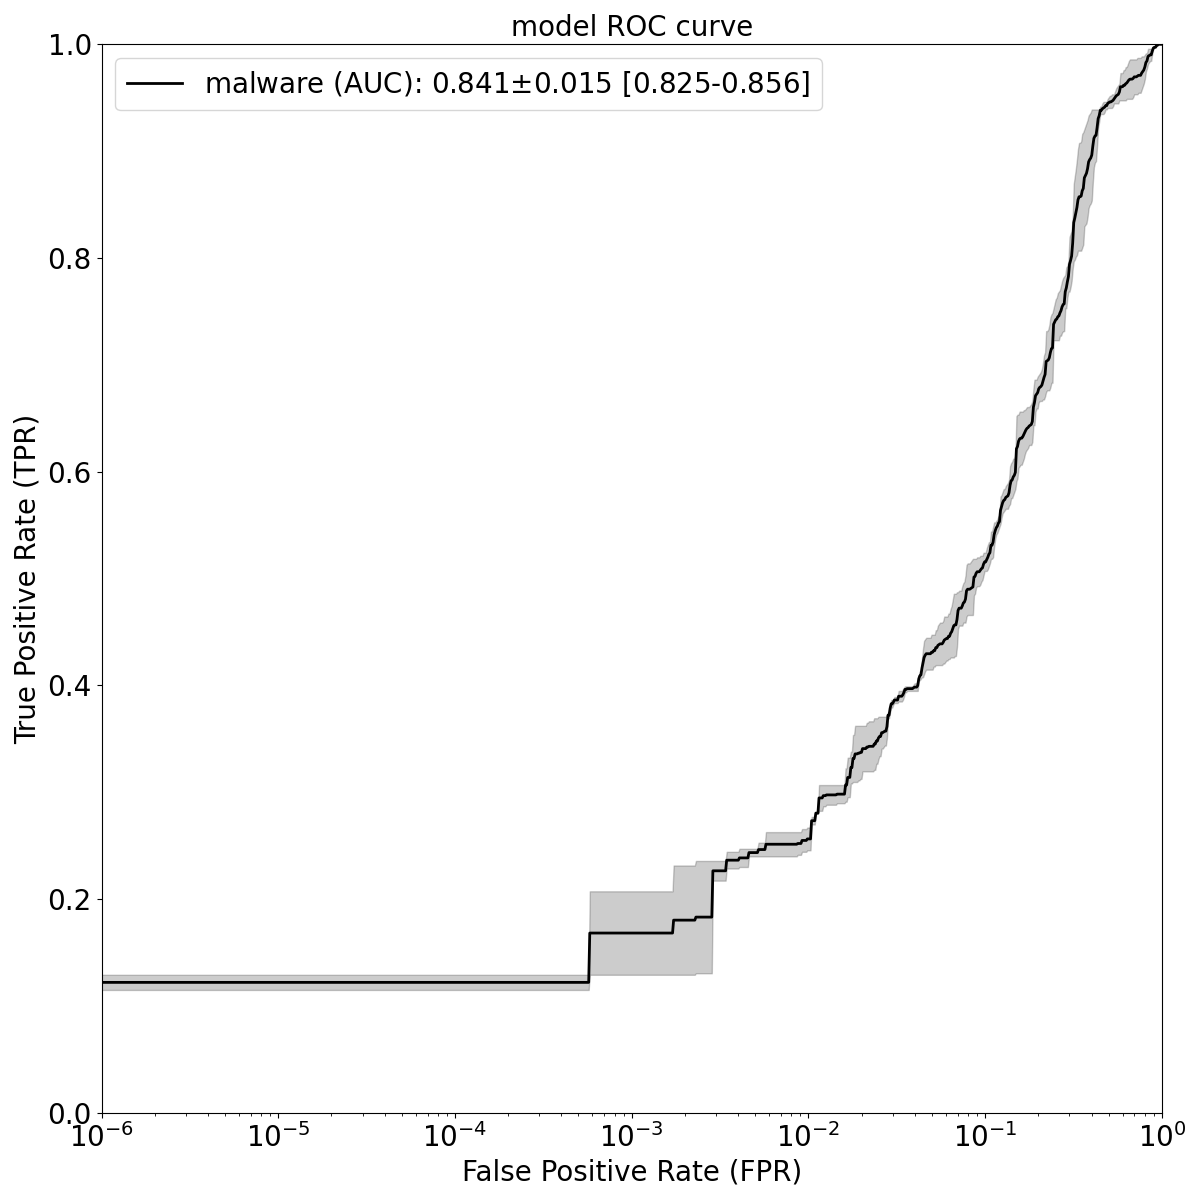
\includegraphics[width=0.6\textwidth]{./results/malware_roc_alohaMB.png}
        \vspace*{-0.2cm}
        \caption[Malware Label prediction task ALOHA (M/B only) ROC curve]{ROC curve and AUC statistics of \textBF{ALOHA (M/B only)} model for the \textbf{Malware Label}. The line represents the \textit{mean} TPR at a given FPR, while the shaded region represents the \textit{standard deviation}. Statistics were computed over \textBF{2} training runs, each with random parameter initialization.}
        \label{fig:malwareRocAlohaMB}
    \end{figure}
}

\newcommand{\malwareRocAloha}{
    \begin{figure}[H]
        \vspace*{-0.5cm}
        \centering
        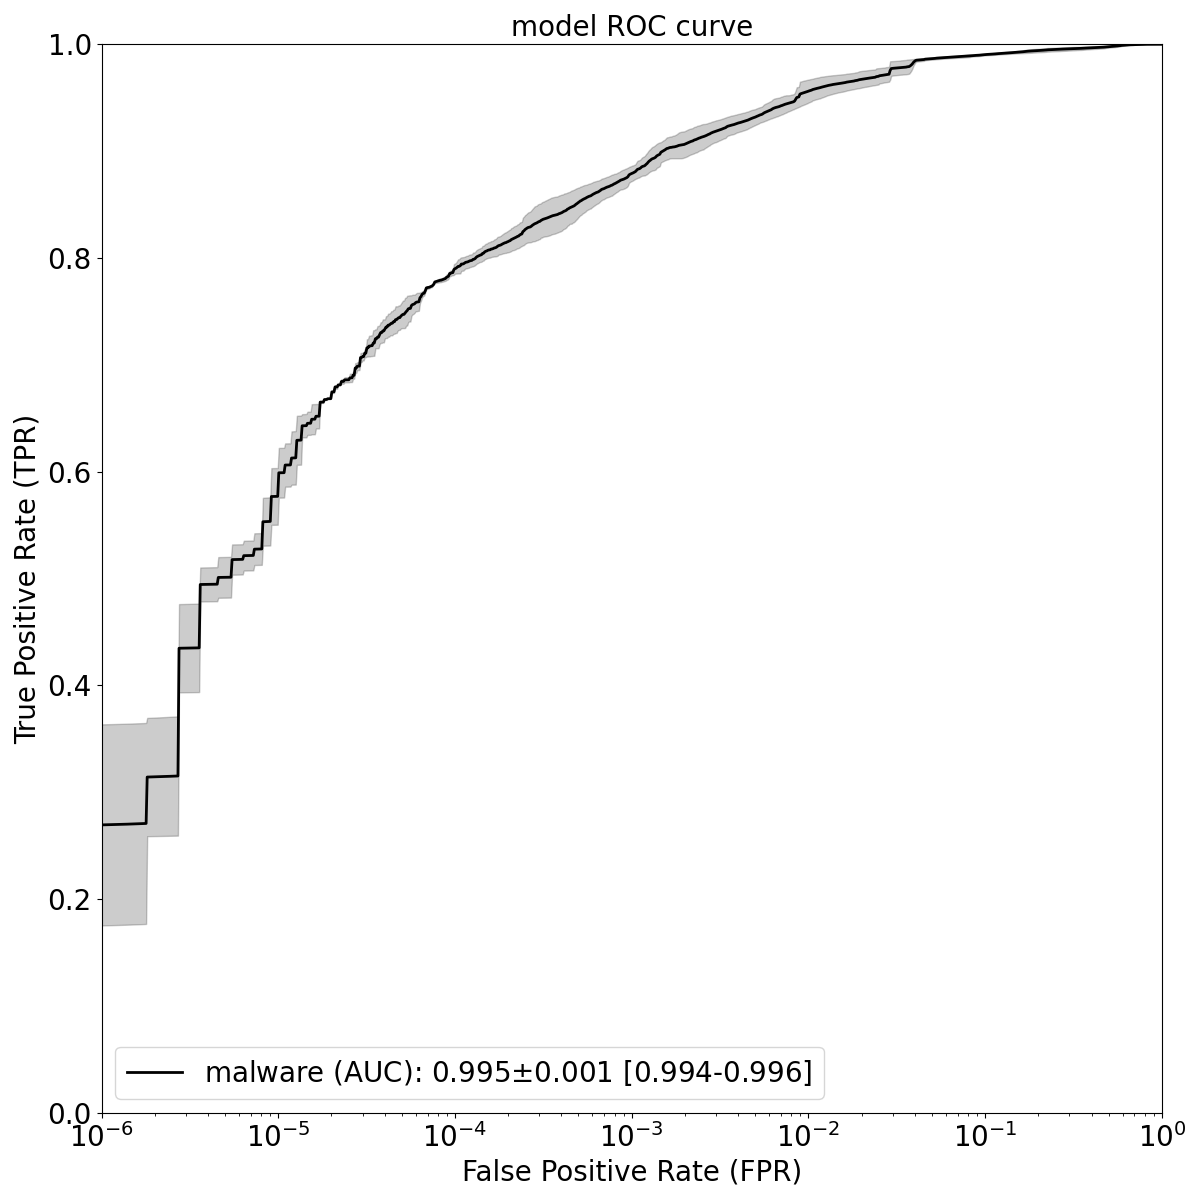
\includegraphics[width=0.6\textwidth]{./results/malware_roc_aloha.png}
        \vspace*{-0.2cm}
        \caption[Malware Label prediction task ALOHA ROC curve]{ROC curve and AUC statistics of \textBF{ALOHA} model for the \textbf{Malware Label}. The line represents the \textit{mean} TPR at a given FPR, while the shaded region represents the \textit{standard deviation}. Statistics were computed over \textBF{2} training runs, each with random parameter initialization.}
        \label{fig:malwareRocAloha}
    \end{figure}
}

\newcommand{\malwareRocProposedMethod}{
    \begin{figure}[H]
        \vspace*{-0.5cm}
        \centering
        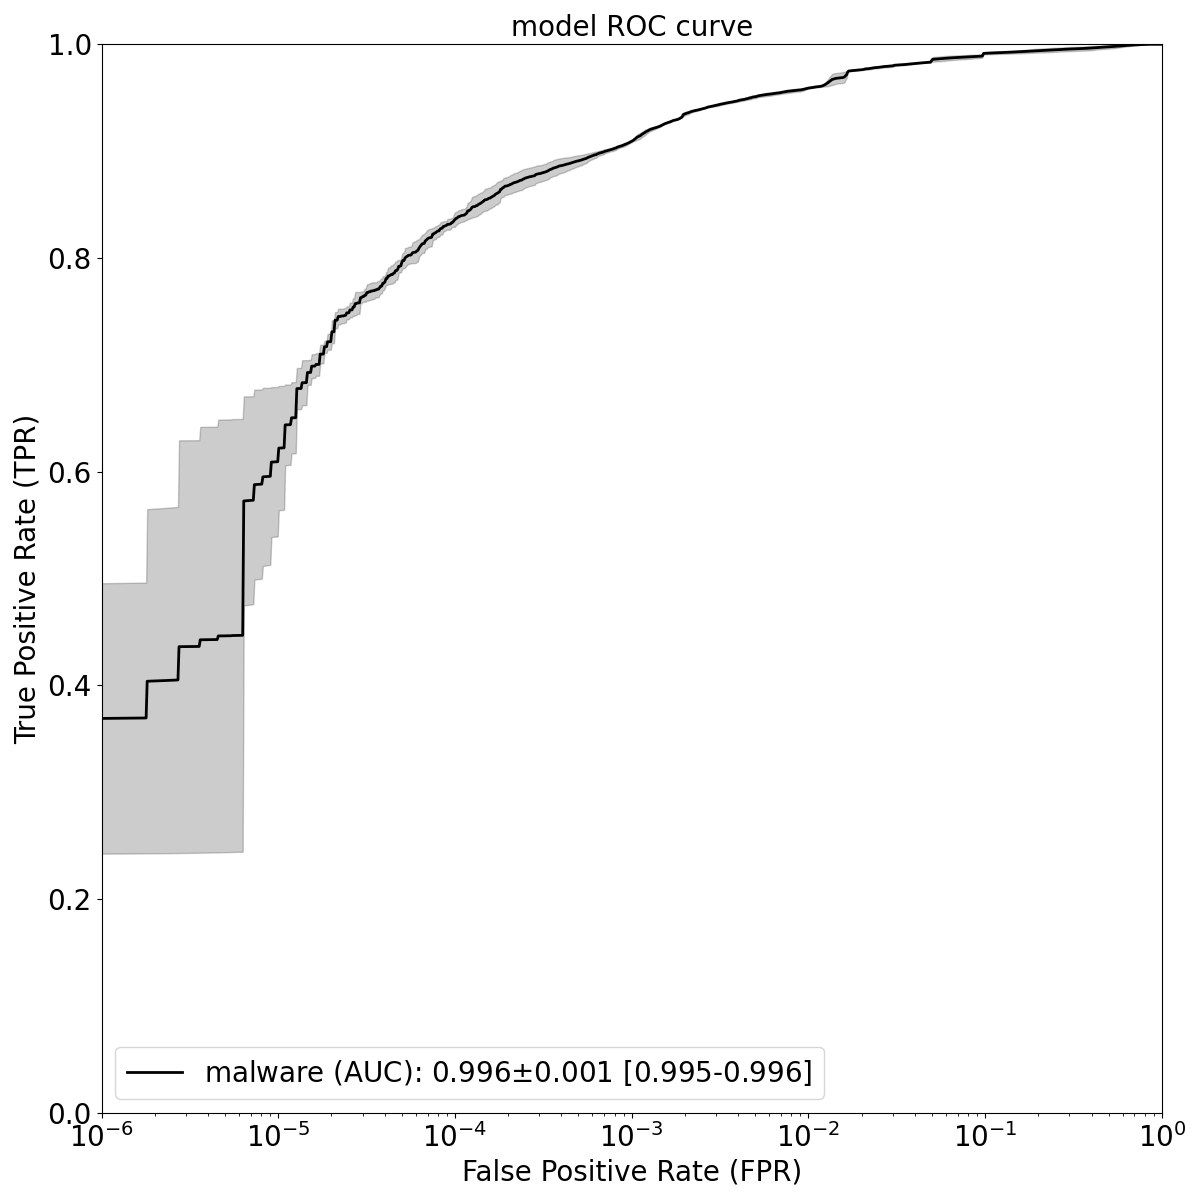
\includegraphics[width=0.6\textwidth]{./results/malware_roc_proposedModel.png}
        \vspace*{-0.2cm}
        \caption[Malware Label prediction task Proposed Model ROC curve]{ROC curve and AUC statistics of \textBF{Proposed Model} for the \textbf{Malware Label}. The line represents the \textit{mean} TPR at a given FPR, while the shaded region represents the \textit{standard deviation}. Statistics were computed over \textBF{2} training runs, each with random parameter initialization.}
        \label{fig:malwareRocProposedModel}
    \end{figure}
}
